    \documentclass[authoryear,preprint,review,12pt]{elsarticle}


    %% Use the option review to obtain double line spacing
    %% \documentclass[authoryear,preprint,review,12pt]{elsarticle}

    %% Use the options 1p,twocolumn; 3p; 3p,twocolumn; 5p; or 5p,twocolumn
    %% for a journal layout:
    %% \documentclass[final,1p,times]{elsarticle}
    %% \documentclass[final,1p,times,twocolumn]{elsarticle}
    %% \documentclass[final,3p,times]{elsarticle}
    %% \documentclass[final,3p,times,twocolumn]{elsarticle}
    %% \documentclass[final,5p,times]{elsarticle}
    %% \documentclass[final,5p,times,twocolumn]{elsarticle}

    \usepackage{amssymb}
    %% The amsthm package provides extended theorem environments
    %% \usepackage{amsthm}

    %% The lineno packages adds line numbers. Start line numbering with
    %% \begin{linenumbers}, end it with \end{linenumbers}. Or switch it on
    %% for the whole article with \linenumbers.
    \usepackage{lineno}
    \usepackage[colorlinks=true,linkcolor=blue]{hyperref}%
    \usepackage{orcidlink}
    \usepackage[colorinlistoftodos]{todonotes}
    \usepackage{setspace}
    \usepackage{tabularx}
    \usepackage{xltabular}
    \usepackage{longtable}
    \usepackage{booktabs}
    \usepackage{multirow}
    \usepackage{hyperref}
    \usepackage{dirtytalk}
    \usepackage[english]{babel}
    %\usepackage{csquotes}
    \usepackage{microtype}
    %\onehalfspacing %TODO Remove Line before final export
    %Path relative to the main .tex file 
    \graphicspath{ {./Figures/} }

    \journal{Sustainable Cities and Society}
    \begin{document}

    \begin{frontmatter}

    %% Title, authors and addresses

    %% use the tnoteref command within \title for footnotes;
    %% use the tnotetext command for the associated footnote;
    %% use the fnref command within \author or \address for footnotes;
    %% use the fntext command for the associated footnote;
    %% use the corref command within \author for corresponding author footnotes;
    %% use the cortext command for the associated footnote;
    %% use the ead command for the email address,
    %% and the form \ead[url] for the home page:
    %% \title{Title\tnoteref{label1}}
    %% \tnotetext[label1]{}
    %% \author{Name\corref{cor1}\fnref{label2}}
    %% \ead{email address}
    %% \ead[url]{home page}
    %% \fntext[label2]{}
    %% \cortext[cor1]{}
    %% \affiliation{organization={},
    %%             addressline={},
    %%             city={},
    %%             postcode={},
    %%             state={},
    %%             country={}}
    %% \fntext[label3]{}

    \title{FROM TRASH TO DIGITAL TREASURE: URBAN DIGITAL TWINING FOR SOLID WASTE MANAGEMENT}

    \author[Utwente]{Iván Cárdenas-León\corref{cor1}\,\orcidlink{0009-0005-0245-633X}}
    \affiliation[Utwente]{organization={Faculty of Geo-Information Science and Earth Observation (ITC), University of Twente},%Department and Organization
                addressline={Hallenweg 8}, 
                city={Enschede},
                postcode={7522 NH}, 
                state={Overijssel},
                country={Netherlands}}

    \cortext[cor1]{Corresponding author}
    \ead{i.l.cardenasleon@utwente.nl}
    %\credit{Conceptualization, Data curation, Investigation, Formal Analysis, Visualization, Methodology, Software, Writing - original draft}

    \author[Utwente]{Mila Koeva\,\orcidlink{0000-0001-7612-5270}}
    %\credit{Supervision, Project administration, Writing - review \& editing}
    \author[Utwente]{Pirouz Nourian\,\orcidlink{0000-0002-3817-7931}}
    %\credit{Supervision, Writing - review \& editing}
    \author[UPretoria]{Calayde Davey\,\orcidlink{0000-0001-9249-5829}}
    %\credit{Conceptualization, Data curation, Supervision}

    \todo{Hide Authors, Double blind}

    \affiliation[UPretoria]{organization={Department of Architecture, Faculty of Engineering, Built Environment and Information Technology, University of Pretoria},%Department and Organization
                addressline={Private Bag x 20}, 
                city={Hatfield},
                postcode={0028}, 
                state={Gauteng},
                country={South Africa}}

    \begin{abstract}
    \label{sec:abstract}
    Urban sustainability faces a critical challenge in managing solid waste. With over 2 billion metric tons generated annually, global waste production has severe health and environmental consequences. Though not a primary SDG, effective waste management is vital for meeting targets 11.6, 12.4, and 12.5 and is intertwined with 12 out of 17 SDGs. South Africa, in particular, grapples with significant waste generation and inadequate collection services. A dynamic model is proposed to tackle these issues, integrating real-time monitoring, optimized collection routes, and citizen participation. This study introduces a prototype for a Waste Management Digital Twin, involving stakeholder prioritization, citizen engagement via an open-source tool (Epicollect5) for locating waste containers and littering sites, waste generation simulations, optimized collection routes, and a control dashboard. Waste generation simulations inform waste flows, low-capacity areas, and optimal container locations. Optimized collection routes are proposed to reduce fuel use and emissions. A control dashboard was developed where stakeholders' system requirements were included, and eleven indicators were displayed along three maps. Stakeholders rated the dashboard high, but some did not perceive the overall objective of digital twinning solid waste. The performance of the Digital Twin depends on computer capacity and local or online processing. The prototype sets the foundation for digital twinning in waste management, scalable to different areas, vehicles, and production levels. Digital twinning, citizen involvement, and multi-stakeholder engagement enhance waste management, particularly benefiting resource-limited countries.
    \end{abstract}

    %TODO: Get Graphical abstract and Highlights
    % %%Graphical abstract
    % \begin{graphicalabstract}
    % \todo{add Graphical Abstract}
    %     %\includegraphics{grabs}
    % \end{graphicalabstract}

    % %%Research highlights
    % \begin{highlights}
    % %\todo[inline]{add Highlights}
    % \item Research highlight 1
    % \item Research highlight 2
    % \end{highlights}

    \begin{keyword}
    %% keywords here, in the form: keyword \sep keyword
    Digital Twins \sep Solid Waste Management \sep Citizen Science \sep Volunteered Geographical Information (VGI) \sep Vehicle Routing Problem (VRP)
    \end{keyword}   
    \end{frontmatter}

    \linenumbers
    %% main text

    \section{Introduction}
    \label{sec:Intro}
    This paper presents a continuation of the work originally presented in The 18th 3DGeoInfo conference \citep{cardenasivanSolidWasteVirtualWorld2024}. Here, we explore the integration of urban digital twin technology with solid waste management systems to address the challenges of waste collection, intermittence, and illegal dumping in urban environments.

    The term urban digital twin (UDT) refers to a digital replica of some of the physical assets of a district or neighborhood of a city that can be used to co-create and test scenarios with city-specific parameters \citep{Ruohomaki2018}. It goes beyond the static 2D or 3D representation, becoming a model for the past, present, and future state \citep{geohubDigitalTwinningUrban2022}. Digital twinning aims to provide laboratory mechanisms for understanding the spatial dynamics and the impacts of climate change, biodiversity loss, permeability, unsustainable transport, and effects of anthropogenic impacts on the city environment \citep{caprariDigitalTwinUrban2022}. An urban digital twin falls within the Augmented Urban Planning framework for strategic planning \citep{Azadi2023} and can work as a Decision Support System to inform urban planners and designers of the impact a project development will have and be a driver for citizen involvement in the planning process \citep{Dembski2019, Dembski2020}.

    Urban digital twins have a process of data feeding - information response – implementation reaction cycle that can move in near-real time and can operate as Urban Computing workflows based on web communication and processing \citep{Nourian2018}. In the first step of feeding data in the cycle, cities are turning to the use of the Internet of Things – IoT for data collection \citep{abadiaSystematicSurveyInternet2022} using sensors that communicate through technologies such as Wi-Fi, mobile networks - 3G/4G/5G-, 6LoWAN, Bluetooth, Radio or NFC \citep{Balaji2019} to address challenges such as air quality \citep{Mak2021}, traffic management \citep{Ibrahim2022}, parking occupancy, or parking restrictions \citep{latreCityThingsIntegrated2016} while leaving other city challenges behind.

    Solid waste management is one of these challenges, which has been identified as important for integrating sensors towards a sustainable city with a significant impact on quality of life \citep{Ismagilova2019}. According to the World Bank, around 2.24 billion metric tons of municipal solid waste were generated in 2020 worldwide \citep{Kaza2021}. A number that has been increased by medical waste during the COVID-19 pandemic in values between 62\% and 350\%, according to  \citep{Yousefi2021}, or between 18\% and 425\%, according to \citep{Liang2021}. Of the overall waste generation, around 33\% of them are not being environmentally safely managed every year \citep{Kaza2018}. 

    The United Nations did not include Solid waste management as a primary Sustainable Development Goal – SDG, potentially reducing its visibility in the political agenda \citep{rodicResolvingGovernanceIssues2017}. However, tackling the issue is intrinsically related to twelve of the 17 SDGs, principally SDGs 11, 12, and 13 \citep{Wilson2015}; therefore, it is a critical task to address to achieve sustainability in cities.

    For the city of Tshwane, the metropolitan municipality surrounding Pretoria – South Africa’s administrative capital – the irregularity of service has led to protests claiming service delivery and consistency at equal levels as of the apartheid white areas of the city \citep{Mokebe2018}. The city reports that the solid waste that reaches the landfill per capita is around 1.95kg/d \citep{tshwaneCityTshwane20222022}, indicating a more significant waste production than the national average. With over six hundred illegal dumping hotspots detected, the city has identified measures to improve the solid waste management system, including confirming illegal dumping sites, allocating new containers, and applying intense cleanup of the streets \citep{tshwaneConsolidatedAuditedAnnual2022}.

    Previous studies have suggested that executing the type of measures, such as the ones identified by the city of Tshwane, requires moving from a traditional static model to a dynamic one that adapts to changes in waste generation and must incorporate real-time container monitoring and frequent collection route optimization \citep{Anagnostopoulos2015a, Hina2020, Ramson2022}. Moreover, the model should include active citizen participation supported by government structures for managing solid waste in a new model of waste governance and sustainability \citep{kubanzaSustainableSolidWaste2020}.

    \todo[inline]{maybe put a paragraph that explains the gap of previous approaches. Although I explain them in the section 1.1}

    In this sense, this paper aims to advance sustainable waste management practices, improve urban cleanliness, reduce environmental impacts, and enhance the overall quality of life in rapidly growing urban areas. This study focuses on the collection stage of the process aiming to create a prototype that incorporates waste generation simulations towards containers and vehicle routing optimization based on the generation and prediction of future volumes. The research is performed in the City of Tshwane, focusing on the Hatfield and Hillcrest neighborhoods as a case study. The research aims to create the first South African digital twin model for solid waste management and propose a prototype that might be replicated in other cities.

    \subsection{Background}
    \label{subsec:Background}
    \subsubsection{Solid Waste Monitoring}
    \label{subsubsec:Monitoring}
    Several sensor implementations have been designed for monitoring solid waste containers. Some include the use of ultrasonic sensors on the lid of the containers \citep{Chaudhari2018, Joshi2022, Karthik2021, Mahajan2017, Ramson2017}, weight sensors at the bottom of the container \citep{Rovetta2009}, a mix of both \citep{Ali2020, Vicentini2009} or infrared sensors \citep{Singh2016}, to detect the status of the containers in terms of fullness capacity. The ultrasonic sensor designs of these studies were only tested at the prototype level, including some indoor simulations of the solid waste collection, which is later reported to a centralized system but tested in no more than two containers. This type of sensor still needs to be tested in specific outdoor conditions of the city where it should be implemented and on a scale that it can be installed in several containers and send the signals to a centralized system that the municipality or company in charge of the solid waste collection of a city can operate. Nonetheless, \citet{Ali2020} simulations demonstrated the possibility of creating production records and using them to forecast daily generation levels for each container.

    While the studies of Rovetta et al. and Vicentini et al. have tested them outdoors, in Shanghai, PR China, with controlled scenarios for residential and commercial usages, the test made by these authors used operators for the containers. It invited citizens to use those particular containers creating a bias in the actual values of on-site generation. These studies already propose including a route optimization for solid waste collection as a future development and use of the designed sensors. In addition, they do not implement them with real-time information.

    The city of Utrecht, Netherlands, has already incorporated ultrasound sensors and daily rerouting based on the level of fullness containers have, reducing the number of vehicles and preventing overflow of the containers \citep{utrechtUndergroundContainersMunicipality2021}, showing the capabilities that this type of integration have on the minority world.

    \subsubsection{Routing optimization}
    \label{subsubsec:routing}
    Solid waste collection can be seen as an inversed good distribution problem, where items must be gathered instead of delivered. It is necessary to optimize the waste collection route to make an efficient collection. Therefore, solid waste collection is an optimization problem that depends on the number of collection points, the waiting time for load and unloading, and the accumulated distance from the landfill to collection points and between collection points \citep{Sarmah2019}.

    %To solve this problem, is it possible to consider it as a Traveling Salesman Problem (TSP), which considers a single vehicle visiting multiple customer locations (nodes) before returning to the depot, where the goal is to minimize the added arc weights (the connection between locations), either if it is travel time or traveled distance between nodes\citep{Herdianti2021}.

    %In its most straightforward formulation, TSP does not have other restrictions, and the problem only depends on the number of locations and the factor that is being measured. When conditions are added to the problem, such as return to the depot after m nodes have been visited, where $m |(𝑛−1)$; or including several deliverables at every node, the variations are known as TSP generalizations \citep{Dantzig1959}.

    %In the solid waste collection scenario, it is necessary to include both the conditions mentioned above, as each node has some goods to collect, and the collection vehicle can only visit a limited set of locations before returning to a landfill. Therefore, the TSP transforms into a generalization known as a Vehicle Routing Problem (VRP) that differs from TSP as there is not only one route but multiple possible routes that require visiting all nodes \citep{Herdianti2021}.

    %As collection vehicles have a limited capacity for carrying goods (waste), their capacity is not uniform, and all node demands are known but variate from node to node; the problem transforms into a combination of Bin Packaging Problem (BPP) and VRP known as Capacitated Vehicle Routing Problem (CVRP) \citep{Herdianti2021, Ralphs2003}.

    Route optimization has been studied for several years with different approaches. The first one is algorithm improvement, where a mathematical method is analyzed to get the most efficient collection route \citep{erdincRouteOptimizationElectric2019, Hannan2018, Sahib2021}, showing the possibility of reducing cost based only on the length of the road segments, and how efficiency also implies an additional coverage of for collection due to the extended use of vehicle fuel. A second approach is agent-based modeling, which simulates the generation of solid waste and sequential filling of containers collected on the shortest route between filled containers, maximizing profits for the collection scheme \citep{Likotiko2017}. On a third method, GIS analysis using the ArcGIS Network Analysis tool has been implemented considering the length of routes, topography, and time taken for collection \citep{Hemidat2017, Jovicic2010, Malakahmad2014}. Finally, an integration of the three methods has been studied, optimizing the route by a mathematical model, including the road network, traffic data, and collection scheme from GIS data, and testing the model in agent-based model simulation \citep{nguyen-trongOptimizationMunicipalSolid2017}. These optimizations follow the same vehicle routing problem: 1) where the route should start and end at the depot or landfill, 2) each container is served by only one route, 3) the vehicle capacity limits the collection, and 4) the route must comply with the traffic regulations of each country.

    The approaches used for vehicle route optimization have shown reduced operation time and savings in fuel and man resources. Only the study performed by \citet{Likotiko2017} considers consecutive optimizations based on the volume of the container and the constant changes in the generation of solid waste that would require re-optimizing the route when including real-time data. These optimizations aim to deliver a one-fit-for-all solution rather than adapting to the requirements of each area and the dynamic generation of solid waste.

    \subsubsection{Stakeholder identification and classification}
    \label{subsubsec:stakeholders}
    As waste management systems include technological, political, environmental, and socio-economic aspects that are interrelated and dynamic, they have many stakeholders \citep{Zaman2011}. Understanding the stakeholders’ characteristics, local conditions, and constraints helps increase participation and improve the effectiveness and willingness to find appropriate solutions \citep{Lishan2021, palacios-agundezIntegratingStakeholdersDemands2014}. Therefore, it is necessary to understand who a stakeholder is, their relations among stakeholders in the specific context of a study area, and the particularities of what is at stake \citep{Freeman2010}.

    One of the methods for stakeholder identification, developed by \citet{Mitchell1997}, introduced a stakeholder classification system based on three attributes: Power, Urgency, and Legitimacy. This framework yields seven stakeholder typologies, Dormant  Discretionary and Demanding (when having one attribute), Dominant, Dangerous and Dependent stakeholders (when having two of the attributes), culminating in Definitive stakeholders with all three attributes (see Figure \ref{fig:graph1}). This classification recognizes latent stakeholders and delineates their roles and limitations.
    \begin{figure}[h]
        \centering
        %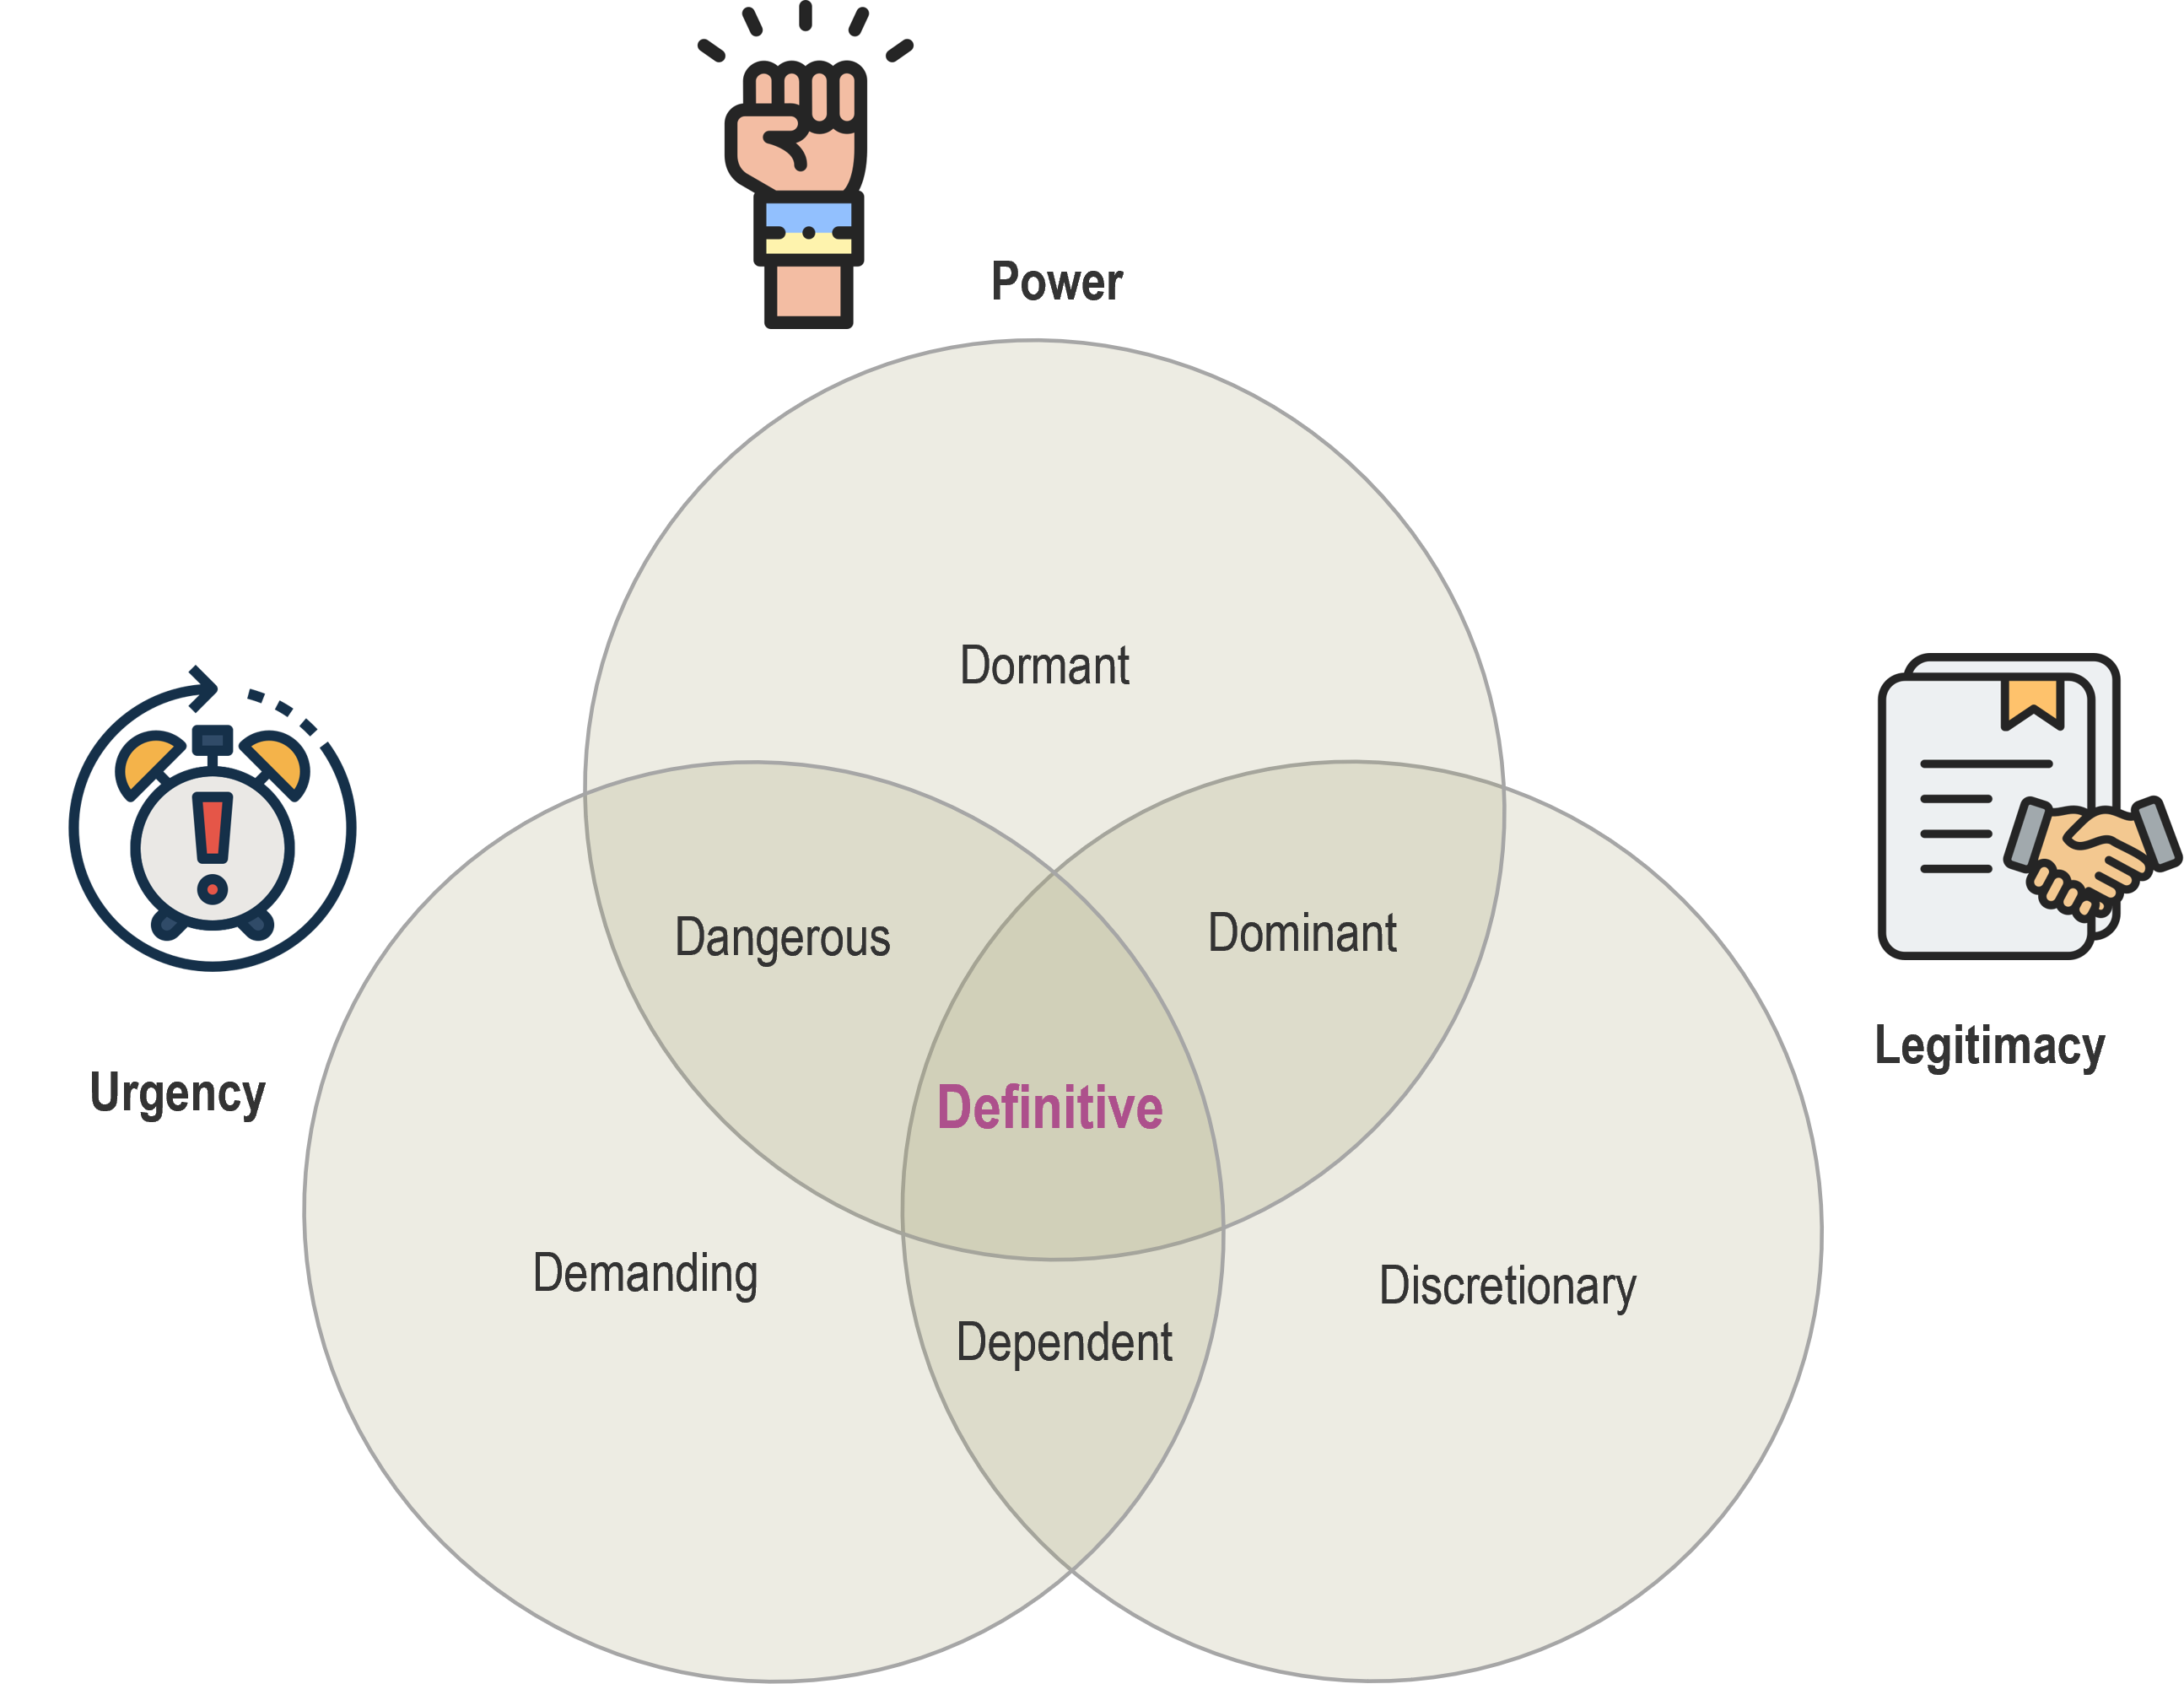
\includegraphics[width=\columnwidth]{Stakeholders Mitchel.png}
        \caption{Stakeholders Typology. One, two or three attributes are present. Source: Mitchel et al. (1997)}
        \label{fig:graph1}
    \end{figure}

    While Mitchell et al.'s model is comprehensive, critics argue it overlooks vulnerable stakeholders lacking any of the three attributes \citep{Shafique2022}. \citet{Driscoll2004} suggest extending the model by incorporating spatial and temporal dimensions, emphasizing physical and social proximity as attributes influencing stakeholder relationships. \citet{Shafique2022} address this gap by introducing proximity as an independent attribute coexisting with power, urgency, and legitimacy. They propose eight new typologies (see Figure \ref{fig:figure2}), expanding the stakeholder classification model and focusing on project operations beyond organizational management, thereby identifying and categorizing vulnerable stakeholders.
    \begin{figure}[h]
        \centering
        %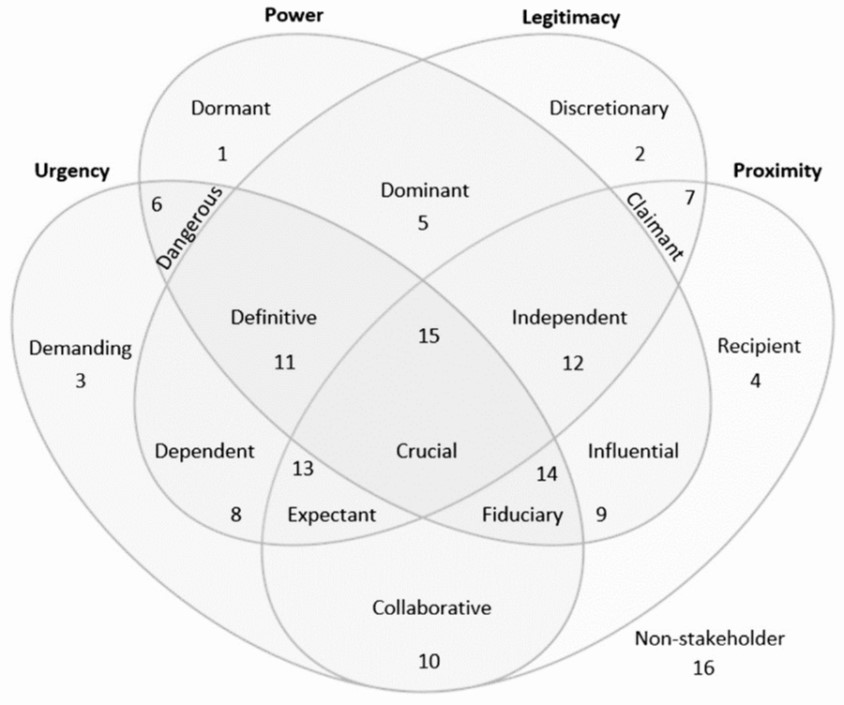
\includegraphics[width=\columnwidth]{Stakeholders shafique.jpg}
        \caption{Stakeholders’ typology with four attributes and their relationships. Source: (Shafique \& Gabriel, 2022)}
        \label{fig:figure2}
    \end{figure}
    % \begin{table}[h]
    %     \label{tab:table1}
    %     \centering
    %     \caption{Stakeholders' Typology, attributes, and description. Source: Shafique \& Gabriel (2022)}
    %     \todo[inline]{not sure if all of this is necessary for the paper or better just to show the image}
    %     \begin{tabularx}{\columnwidth}{l X X}
    %         \toprule
    %         \#  & New Typology (Attributes) & Description \\
    %         \midrule
    %         4   & Recipient (Proximity) & Recipient stakeholders receive some benefit from the project because they reside in or close to the project implementation area. Although not the project’s target beneficiaries, they benefit indirectly from the project because of their physical closeness to its beneficial outcomes. \\
    %         7   & Claimant (Legitimacy \& Proximity)    & Claimant stakeholders have a perceived legitimate role and claim to the project and reside in or close to the project area. They receive a direct benefit from the project outcomes. \\
    %         9   & Influential (Power \& Proximity)  &  Influential stakeholders are powerful and either reside in or have some form of control over the project implementation area. \\
    %         10&Collaborative (Urgency \& Proximity) & Collaborative stakeholders do not possess power and legitimacy. However, because they were affected by the disaster due to their closeness to affected areas, they have a high interest in the urgent completion of the reconstruction project. Their collaboration contributes to the success of the project. \\
    %         12 & Independent (Power, Legitimacy \& Proximity) & Independent stakeholders can implement the project without the help of other stakeholders because of their ability to influence others and the official recognition of their role in implementation. These are usually local stakeholders with a physical presence in the project area \\
    %         13 & Expectant (Legitimacy, Urgency \& Proximity) & Expectant stakeholders are not considered powerful but expect to benefit directly from the project because they possess urgency, proximity, and legitimacy attributes. Other stakeholders (though not necessarily project implementers) recognize them as stakeholders, legitimizing their role. \\
    %         14 & Fiduciary (Power, Urgency \& Proximity) & If collaborative stakeholders acquire power over the project implementation area, they become fiduciary stakeholders. Project managers recognize their responsibility to report directly to these stakeholders on project outcomes. Vulnerable-affected communities might aspire to this role by demanding community-driven approaches to project implementation. \\
    %         15 & Crucial (Power, Legitimacy, Urgency \& Proximity) & Crucial stakeholders are the decision-makers, implementers, and beneficiaries of the project. Possession of proximity attributes helps them to gain direct benefit from the project. For vulnerable affected communities, the role of a crucial stakeholder is even better than that of a fiduciary stakeholder.\\
    %         \bottomrule
    %     \end{tabularx}
    % \end{table}
    Although the model provides a comprehensive identification and classification system, just as Mitchell et al., the newly suggested model does not consider a method for identifying the possession of each attribute and the relationships between one and another stakeholder. Therefore, the classification tends to be subjective to the researcher's interpretation creating a significant bias on the typology allocation.
    \section{Methods} \label{sec:Methods}
    \subsection{Data} \label{subsec:Study Area}
    The study focused on the Hatfield and Hillcrest neighborhoods of the capital city of South Africa, Pretoria. The area comprises 9.45 km$^2$ surrounding the University of Pretoria main campus (See Figure \ref{fig:studyArea}) with different land uses such as residential, institutional (embassies), commercial, agricultural, and educational. This area is part of the ongoing project of African Future Cities from the Department of Architecture in the Faculty of Engineering, Built Environment, and Information Technology of the University of Pretoria. The area also includes the Hatfield City Improvement District (CID). This non-profit and private organization performs corporate governance of the area. It is funded by a taxpayer’s property levy collected by the municipality and transferred to the Hatfield CID for operation, providing additional services such as cleaning and maintaining public spaces, private security, and urban embellishment \citep{cidHatfieldCIDBrochure2021}.
    \begin{figure*}[h]
        \centering
        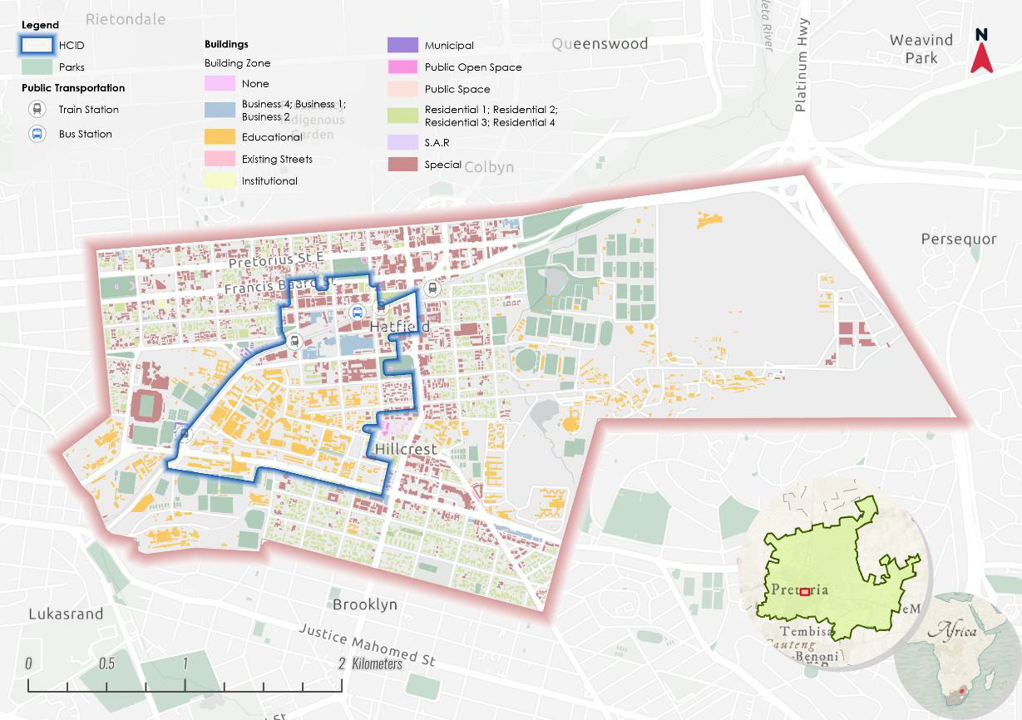
\includegraphics[width=\linewidth]{studyAreaHatf.png}
        \caption{Hatfield Digital Twin City Study Area.}
        \label{fig:studyArea}
    \end{figure*}
    \subsection{Geospatial Datasets} \label{subsec:Geospatial}
    The research was supported with geospatial data from the City of Tshwane, the National Geo-Spatial Information Centre of South Africa, and data collected by the Faculty of Engineering, Built Environment, and Information Technology of the University of Pretoria. The initial data required for the research are summarized in Table \ref{tab:Datasets}, including data type and sources of information. To use in a web environment, all data was reprojected to WGS 1984 (ESPG: 4326). Nonetheless, length and area attributes were calculated in Hartebeesthoek94 / Lo29 (ESPG: 2053).

    \begin{table*}
        \centering
        \caption{Datasets used}
        \scriptsize
        \label{tab:Datasets}
        \begin{tabularx}{\linewidth}{X X X X X X}
            
            \toprule
            Geospatial Dataset & Specifications & Data Type & Date & Coordinate System & Source \\
            \midrule
            LIDAR Scanning & Aerial laser scanning with 0.6m of separation & LAS & June,2019&EPSG:4148&University of Pretoria, ESRI \\
            Buildings&Building footprints with attributes Name,type of building&Vector Polygons& March,2023&EPSG: 4326&OpenStreetMaps Contribuitors\\
            Road Network&Polyline of motorcar roads, including total length, road direction, road type&Vector Lines&March, 2023&EPSG:2053&City of Tshwane GIS portal\\
            Aerial Imagery&Very High-Resolution Imagery from Unmanned aerial vehicles - UAV from the study area. RGB Bands. 0.1m Spatial Resolution&Raster&June,2018&EPSG:2053&City of Tshwane GIS Portal\\
            Zonning&Polygons DEfining regulations for land use&Vector Polygons&March 2023&EPSG:2053&City of Tshwane GIS Portal\\
            Global Settlement Population&Estimated Residential population per 100x100m cell. Epoch 2020&Raster&June, 2022&EPSG:54009&GHS population grid multitemporal (1975-2030) \citep{Schiavina2022}\\
            Solid Waste Containers and Littering Location&1,270 containers and 820 illegal dumping reports &March,2023&EPSG:4326&Vector Point& On-field data collection - \citep{cardenasivanSolidWasteVirtualWorld2024}\\
            \bottomrule
        \end{tabularx}
    \end{table*}

    \subsection{Stakeholder identification} \label{subsec:stakeholderIdent}
    Based on an unstructured interview with a key informant, a stakeholders’ workshop took place on the 31st of January 2023. The activity focused on understanding the dynamics and relationships of the stakeholders and their expectations and requirements to improve solid waste collection management. Such requirements were asked of the stakeholders, separating them into three categories: Strategic, Operational, and Performance.

    The workshop was video recorded. Authorization of the participants and a transcript were generated using the method developed by \citet{Radford2022}. The text was analyzed by identifying additional stakeholders and the relationships of Power, Urgency, Legitimacy, and Proximity that exist between all of them and classified them according to the typologies of the Salient Model \citep{Mitchell1997, Shafique2022}.

    To perform such classification and reduce the subjectivity, a pairwise comparison was made using the Analytical Hierarchical Process described by \citet{Saaty1987, Saaty1990}. Each attribute was compared on a nine-point scale of their attribute level when stakeholder i is compared with stakeholder \textit{j}, as explained in Table \ref{tab:Saaty}.

    \begin{table*}
        \centering
        \caption{Analythical Hierarchical Process pairwise comparison. Source: (T. L. Saaty, 1990)}
        \small
        \label{tab:Saaty}
        \begin{tabularx}{\linewidth}{X c}
            \toprule
            Relative Importance&Definition – X: power, urgency, legitimacy, proximity\\
            \midrule
            1&\textit{i} and \textit{j} have equal X\\
            3&\textit{i} have moderate X over \textit{j}\\
            5&\textit{i} have strong X over \textit{j}\\
            7&\textit{i} have very strong X over \textit{j}\\
            9&\textit{i} have extreme X importance over \textit{j}\\
            2,4,6,8&Intermediate values between two adjacent judgments\\
            Reciprocal&When the relation is inverse –
            (eg. \textit{j} has strong X over \textit{i}: 1/5)\\
            \bottomrule        
        \end{tabularx}
    \end{table*}
    Values are then normalized, and, based on the resultant eigenvector of each attribute, the different stakeholders were classified according to the typologies of the Salience model. On this classification, stakeholders classified as \textbf{Definitive} and \textbf{Crucial} were considered the primary end users of the Digital Twin.

    \subsection{Urban Waste Management Digital Twin Design} \label{subsec:Phase3}
    The design of the Urban Digital Twin comprehends a series of steps as city reconstruction, waste calculation, route optimization, and system integration. In Figure \ref{fig:flowchart}, there is a detailed flowchart that summarizes the process.

    \begin{figure*}
        \caption{Urban Digital Twin Design Flowchart.}
        \label{fig:flowchart}
    \end{figure*}

    \subsubsection{System Architecture and Data integration}\label{subsubsec:SystemArch}
    Integrating the elements in one Digital Twin tool followed the architecture proposed in Figure \ref{fig:architecture}. To create an online, easily accessible control tool, a Dashboard was developed, including the stakeholders’ user requirements identified in section \ref{subsec:stakeholderIdent}.
    \begin{figure*}
        \caption{Waste Digital Twin Architecture}
        \label{fig:architecture}
    \end{figure*}
    The process includes retrieving citizens' collected data through Epicollect5 API that is exported to a JSON file, filtered, and transformed into a CSV point file that can be converted to a point layer to display the containers. Then, the container allocation for buildings is assigned using a near function. The optimal route is calculated, and the resulting route and pick-up sequence are displayed in an operational Dashboard where layers on the dashboard are updated every 6 seconds. The dashboard contains descriptive statistics and the key elements identified by stakeholders.

    \subsubsection{City Buildings reconstruction}\label{subsubsec:Buildings}
    An aerial LIDAR scan from Jun 2019, with a spatial accuracy of 60cm, was classified into five categories: ground, noise, low vegetation, high vegetation, and building points. OpenStreetMaps – OSM – building footprints \citep{contributorsPlanetDumpRetrieved2023} were used to help the building classification by performing a 2D intersection that differentiated the vegetation from the buildings.

    Later, the building points were transformed into a flat raster (no Z values) where void areas were filled in at a distance of 1.2m (double the pixel size). The resulting raster was transformed into polygons on which edge angles were normalized into right angles and diagonals to obtain geometrically valid polygons. The final polygons were, once again, compared with the OSM to extract the footprints that the OSM contributors had not mapped. Both footprints were merged into a single file containing the complete building footprints of the study area. The quality of the result was tested with a confusion matrix analyzing 1,000 random point locations in the study area. To improve quality, identified polygons with areas smaller than 25 $m^2$ and heights \> 3m were inspected visually to detect and eliminate false positive results that generally were related to trees.

    With the ground classification of the LIDAR point cloud, a Digital Terrain Model, Digital Surface Model, and Normalized Digital Surface Model were generated. Together with the building footprint, these were used to extract the base elevation of the buildings, average height, and rooftop form by classifying them as Flat, Shed, Gable, Hip, Mansard, Dome, Vault, or Spherical. This classification is used for the 3D representation of the roofs and to apply procedural textures.

    The attributes number of stories above ground, class, function, and usage from the CityGML 3.0 model were used to have more extensive information on the building's attributes. The data for each building was obtained by combining OSM information, City of Tshwane zoning \citep{tshwaneGeographicInformationSystem2023}, and on-field validation of the attributes. This validation was performed by a group of 76 first-year Architecture students at the University of Pretoria. Additionally, for each building, the total floor area was calculated by dividing the height into 2.4 meters – The minimum required height for rooms in Tshwane \citep{tshwaneTshwaneTownplanningScheme2014} – and multiplying this value for the footprint area to obtain the total floor area. A UAV Image was used to perform quality control in classifying buildings and determine their usage where on-field validation was not possible.

    \subsubsection{Solid waste generation calculation} \label{subsubsec:Generation}
    To obtain an estimation of the population residing in each building of the study area, it was employed the Global Human Settlement Population Layer \citep{Schiavina2022} on a 100m resolution calculating the population density for each pixel based on the total floor area of residential buildings inside each polygon. The population density value mentioned above was used to derive the population count for each residential building. The resulting inhabitants’ calculation was then multiplied by the average waste production value, allowing us to estimate the daily waste production per building.

    Non-residential buildings were categorized into four classes with production per class as described in Table \ref{tab:waste1}. These categories are organized from higher to lower generation rates, and the waste production corresponds to the upper tier of the range indicated for each class by \citet{Karadimas2008}.

    \begin{table*}[h]
        \centering
        \caption{Building Classes, related commercial activity, and Waste production. Source: Adopted from (Karadimas \& Loumos, 2008)}
        \small
        \label{tab:waste1}
        \begin{tabularx}{\linewidth}{l X c}
            \toprule
            Category&Typical Commercial Activity&Waste production 
            $(kg/(m^2)d)$\\
            \midrule
            A&Supermarket, bakery, restaurant, grocery store, greengrocery store, fish store, fast food, bar, pub, club, café.&0.419\\
            B&Butcher store, patisserie, hairdresser, wine-vault, floristry, garage, pizzeria.&0.225\\
            C&Theatre, church, school, bookstore, barbershop, traditional café, pharmacy, post office, lingerie.&0.124\\
            D&Embassy, office, Insurance company, chapel, betting shop, tutoring center, shoe store, clothing store, jewelry store, video club.&0.024\\
            \bottomrule        
        \end{tabularx}
    \end{table*}

    For each building, the closest container, on an “as crow flies” method, was assigned to indicate where solid waste might be deposited and collected. A 600kg/m3 waste density was also assigned as the collection company's operational estimation for its current routing scheme. To simulate the waste production at each location, a random number between 0 and 1/24th of the total daily production was generated, where a maximum excess of the daily production was set to 20\%.

    \subsubsection{Optimal Collection Route} \label{subsec:OptimalR}
    A network analysis was performed using a Capacitated Vehicle Routing problem solver \citep{ESRI2023c} to calculate the optimal collection route. The model for the route solution included several factors, such as the aggregated containers’ location, their current volume to be collected, the saturation, and limitations by vehicle capacity.

    The solver uses a nearest insertion heuristics algorithm combined with the Tabú search metaheuristic method from ESRI for solving the CVRP \citep{ESRI2023a}. This type of algorithm explores solutions by moving from a solution to a neighbor solution, even accepting a temporal detriment on the current iteration, to find a better global result (Local Search) \citep{Avdoshin2019, Laporte2014}. In the nearest insertion, the problem solution selects the shortest edge and performs a sub-solution of it, then selects a node not in the solution with the shortest edge to create consecutive nodes; it follows by finding an edge where the insertion of the consecutive nodes will be the minimal accumulation between previously solved nodes \citep{Nilsson2003}. The Tabú search method allows moves with a negative gain if a positive has not been found. The algorithm creates a list of illegal moves to avoid infinite circular loops. Once a neighboring solution is chosen, it will be added to the tabu list, ensuring that it is not revisited unless it leads to an improved tour or is removed from the list (\textit{ibid}).

    For this study, first, the road vector layer was classified to identify monodirectional and bi-directional segments. Their category (residential, highway, link) and the speed of vehicles are restricted to transit. The second step includes creating a Network analysis layer and identifying edges and nodes. Here, each edge weight was calculated according to the time needed to travel the road segment using each segment's maximum speed and length.

    The third step corresponds to selecting such containers where saturation is higher than 75\% (this is an arbitrary value that was selected as ¾ of the capacity of the container) and loading them in the network as collection orders. 

    Following this, the conditions of analysis are configured including the starting and ending Once the network is configured, waste is accumulated as described in the previous section, and the problem-solving process occurs every sixth iteration (skipping the 24th one to represent night and non-working collection hours), using a method developed by ESRI. The process starts by creating an OD matrix representing the shortest path between the collection orders and the landfill location. Collection orders are added one at a time to the best route, and the process is enhanced on a tabu search metaheuristic approach to finding an optimal solution \citep{ESRI2023c}.

    Once the solution has been found, inserted containers’ current waste and saturation are reset to zero, representing a clean-up or collection of the containers. Meanwhile, the non-collected orders keep accumulating until their saturation reaches the threshold. After each clean-up, routes, and orders are deleted to make space for the new route and avoid memory overload.

    \subsection{Stakeholder Assesment} \label{sub:MethAssesment}

    On the 12th of July 2023, A workshop demonstration of the Urban digital twin was performed with 21 stakeholders showing them the possible interactions and data that can be visualized and operated in the digital twin control dashboard. The overall development process of the digital twin was shown to the attendants along with a Demo video (See \href{https://www.youtube.com/embed/6k209psuRqw}{Youtube link}) of the functionality. They could use the tool freely after the video, and a questionnaire was delivered to the participants to evaluate the prototype.

    The questionnaire was designed with questions on a five-point Likert scale aiming to evaluate the user’s satisfaction (see \ref{apendix}) \todo{should I include the questionare as an annex??}. It measures the usability and usefulness following the method proposed by \citet{Ballatore2020} and the added value analysis proposed by \citet{Pelzer2014}at the group and outcome levels (See Figure \ref{fig:AssesmentFr}). The evaluation of the Digital Twin was analyzed and discussed following the Gemini Principles \citep{aGeminiPrinciplesGuiding2018} in their three classes: purpose, trust, and function (Figure \ref{fig:DTPrinciples}).

    \begin{figure}[h]
        \caption{Assessment Framework.
        Source : adaptation (Aguilar et al., 2021 ; Ballatore et al., 2020 ; Pelzer et al., 2014)}
        \label{fig:AssesmentFr}
    \end{figure}

    \begin{figure}
        \caption{Digital Twins Gemini Principles. Source: (Bolton A \& Schooling, 2018)}
        \label{fig:DTPrinciples}
    \end{figure}

    \section{Results}
    \subsection{Current Practices}
    According to the Community survey report of the Province of Gauteng \citep{africaProvincialProfileGauteng2018}, the city of Tshwane had 2,921,488 inhabitants in 2011 and 3,275,152 in 2016. This indicates an average annual growth of 2.28\%. Calculating the value for 2023, with the same growth rate, the city now has an approximated population of 3,835,010 inhabitants.

    As early as 1995, the Gauteng Province recorded an urbanization level of 94\% \citep{serviceLivingGautengSelected1997}. Likewise, the 2011 census shows that the city of Tshwane had an urbanization level of 92.3\% \citep{africaCensus20112012}. Assuming there has not been a considerable change on this level, the total population in the urban area of Tshwane is 3,539,714 inhabitants in 2023. At a rate of 1.95 kg/inhabitant-d \citep{tshwaneCityTshwane20222022}, the overall production is 6,902.44 Tons/day of waste for residential, commercial, and industrial waste.

    The stakeholder workshop provides information to understand the city's collection scheme process. Generally, the municipality collects the waste of residences and businesses once every week on 18m3 compacter vehicles that have an efficiency of 4km/L of Diesel. Each suburb has its designated day, and collection companies only control the type of building and number of residential units in each suburb. Due to their high waste production, restaurants get their waste collected daily. Additionally, individual businesses can contract a private waste collection company to provide the service in their required conditions.
    \begin{quotation}
        \say{\textit{[For] business, there [is] an option or a daily collection as well. It’s a different kind of bin. But, as far as I know, it’s not sorted. It’s not recyclable in terms of the sorting. So, it’s not differentiated, but it’s just a regular collection on a daily basis}}  - CID
        
    \end{quotation}

    The municipality also has a team of foot workers in the public area who deal with pedestrian and vehicle littering. They are provided with bags for picking up the litter, which is then moved to central points where trucks can collect them. Contrary to the truck collection, foot personnel do not work on a scheduled basis. Instead, they do so in an “as the need arises" approach.

    The CID provides a littering picking improved service on the streets, sidewalks, and parks of their service area with 16-foot workers and one truck. For the picking, the municipality provides them with garbage bags of around 70,000 to 80,000 bags of waste yearly, registered by each worker and their supervisor in a manual scorecard log.
    Within the CID, the working schedule for foot workers follows a standardized timetable. From 7 am to 11 am they perform litter picking in their designated area of around 1 to 1.5 blocks. In the afternoon, they would focus on performing tree maintenance and biowaste cleanup. In the case of city events and the CBD – where bars and restaurants are located -or after a weekend, workers would focus on the area where the event took place and continue with their assigned activities. On the other side, private student accommodations, where around 30,000 students live, have their private collection in small trucks.

    \begin{quotation}
        \say{\textit{So we haven’t got to a point where there’s a sort of a connected waste strategy for the full precinct}}- CID
    \end{quotation} 

    The different collectors in the city take the gathered waste to five landfills where waste can be taken. Usually, the waste goes to the closest landfill where collection occurs. In the case of the Hatfield study area, this is the Hatherley Municipal Dumping Site located at 28.407°E - 25.741S (Figure \ref{fig:landfill}).

    In the waste dumping sites, trucks dump their waste in the space indicated by the location supervisor. When the area is getting full is then compacted by a front-end loader. The waste dumping sites are open to the public, where they can discard materials such as construction waste, electrical appliances, or bio-degradable waste.

    \begin{figure*}[h]
        \caption{Hatherley Municipal Dumping Site location in relation to the Study Area}
        \label{fig:landfill}
    \end{figure*}

    \subsection{Stakeholder classification and system requirements} \label{subsec:Classification}

    A total of 15 stakeholders were identified after the stakeholders' workshop. Analyzing the workshop transcript, it was possible to create four pairwise comparison matrices for the four analyzed attributes and classify them in the typologies as seen in Table \ref{tab:stakeholderTyp}. Three of them were identified as non-stakeholders for the Waste Digital Twin prototype: Local Researchers, Student residences and Composte providers.

    \begin{figure*}[h]
        \caption{Stakeholders' attributes and typologies. Attribute values are percental weights for each attribute calculated. Bold numbers indicate the largest weight for each attribute, and blue numbers indicate the lowest weight for each attribute. Typologys highlighted in purple are the stakeholders considered a primary focus for compliance with user requirements.}
        \label{tab:stakeholderTyp}    
    \end{figure*}

    The most powerful stakeholders are related to the political power the Department of Forestry Fisheries and Environment – DFFE - has on regulations and requirements for the provision of the solid waste management service. The regulations imposed lay on the municipality the responsibility for providing the service within their area or government, giving them the power to set up their own rules for service delivery.

    Nonetheless, other stakeholders also have large power in solid waste management as the proximity to the core of waste management reduces. For instance, the landfill operators have gained non-overviewed control of the dumping sites where

    \begin{quotation}
        \say{\textit{All […] points to a total lack of management from the city side. To control that (landfill operation) […] They (landfill operators) don’t look too afraid to go there. All they’re doing is: the trucks are being allowed in, and whatever happens there is being managed on-site and the city keeps applied by, because they know each truck that comes in is already being paid}}
    \end{quotation}

    Apparently, this is due to the economic benefit it implies to operators at the cost of the citizens. As the municipality themselves recognizes:

    \begin{quotation}
        \say{\textit{“… it’s not very good. [Waste] Generation is a lot of income from the city. The income, just by households and businesses pay them. They collect this waste in every place and go and then they dump it in about five landfills in the city}}
    \end{quotation}

    On the urgency side, the CID stakeholder has been identified as the one with more urgency as they provide a local governance service to the community who pay a tax to enhance the neighborhood. So, they want to deliver that promise and respond to the tax contributors. In their own words:

    \begin{quotation}
        \say{\textit{We are friendly with the landlords. I mean they pay me a levy and we want to try and give them the most value for it. So, […] how do we make sure that we manage your waste in a more effective way because they [Business and Offices] waste everything in Box Street right? at the back of the center, and there’s whatever serious smell there you understand? You know the bad smell is a sign of bad management. That’s all it is. So, we need to find a better way of dealing with this thing and say: ‘There’s some clever people around the table who want to help you’ because let’s help each other in this thing so that for me is a very big opportunity}}
    \end{quotation}

    Another stakeholder identified with urgency is the Ward Counselor, as he becomes the key connection point between citizens and the municipality. Complaints of waste collection and littering go through the counselor, and their job gets filled with citizens' complaints when, for instance, waste has not been picked up, as the municipality representative recalls:

    \begin{quotation}
        \say{\textit{[The] majority of ward councilors use WhatsApp systems very, very effectively. That’s the shortest communication. Whether there’s no water, no electricity, that poor council has been bombarded instantaneously. ‘Why is electricity supposed to come on the level? It’s now five minutes past 11, what does it mean?’ The same request.}}
    \end{quotation}

    The key informant also provides insights into how the counselor is this crucial link between communities and how they can benefit from the Digital Twin for waste management:

    \begin{quotation}
        \say{\textit{So, when we are a problem as a domestic or business, and it’s a big problem that I get frustrated with, I send my counselor, and everybody does this, typically the first complaint. I also log my calls with the city to get a record, but usually, the action happens through the WhatsApp group and the counselor who elevates that issue. And that’s how our cities function in a formal way}}
    \end{quotation}

    \begin{quotation}
        \say{\textit{“… if we can advance whatever we’re doing with waste and make that person shine and successful, that’s a political massive value add on both sides of making waste go away or making crime, whatever the issue is. So, I think that’s one of our end users. is can the ward councilor’s job be so much easier and better because of how we are working with waste? That’s a kind of end user.}}
    \end{quotation}

    The legitimacy of the stakeholders is balanced between most of the stakeholders as each has its claim and is recognized by other stakeholders. However, residents become more legitimate as they are affected by the service performance and the effects illegal dumping can have. As the focus of the proposed Digital Twin is only on the collection phase of waste management, landfill operators were given low legitimacy compared to other stakeholders. This is also related to their interest in keeping waste flowing toward the landfill without much control, as explained above.

    Finally, the proximity attribute was higher for the residents and waste pickers as they are in proximate contact with the waste, and any change in the waste management scheme will positively or negatively impact them. On the other hand, the DFFE has the least proximity to the stakeholders as their role is related to national policies and is more distant from local issues and solutions.

    In this way, when organizing the stakeholders in the Salience Model, the CID and Ward councilor have a typology of Crucial as they rank high in all four attributes. The municipality is then characterized as a Definitive Stakeholder as it ranks high in three attributes but has lower proximity than other stakeholders. As explained in the methodology, as a result of the classification, these three stakeholders are the ones that were considered end-users of the Digital Twin tool. Figure \ref{fig:typologies} shows the distribution of the stakeholders on the sixteen possible typologies.

    \begin{figure*}
        \caption{Stakeholders’ typologies for Waste Collection Digital Twin.}
        \label{fig:typologies}
    \end{figure*}

    The stakeholders identified 32 requirements for improving solid waste management: zero waste and assessing environmental impact, the most common. Stakeholders highlighted the importance of aligning to the Sustainable Development Goals (SDGs), the Nationally Determined Contributions (NDC) under the Paris Agreement, and the European Sustainability Reporting – ESG- Standards (Table \ref{tab:initialReq}).

    \begin{table}
        \centering
        \caption{Stakeholder user requirements.}
        \scriptsize
        \label{tab:initialReq}
        \begin{tabularx}{\columnwidth}{X r}
            \toprule
            Category&Elements\\
            \midrule
            \multirow{10}{*}{Strategic} &Carbon footprint reduction\\
                                    &Environmental impact\\
                                    &ESG reports\\
                                    &Polluter Identification\\
                                    &Reports to NDC for Paris Agreement\\
                                    &Scalability to Country\\
                                    &SDG Goals performance\\
                                    &Sources of waste\\
                                    &Type of waste generated\\
                                    &Zero Waste\\
        \midrule
        \multirow{8}{*}{Performance}&Dedicated person-hours\\
                                    &Optimally used container's location\\
                                    &Recycling per building\\
                                    &Recycling per campus (university)\\
                                    &Recycling per sorting area\\
                                    &Total Generation Waste\\
                                    &Trucks Fuel consumption\\
                                    &Waste production heatmaps\\
        \midrule
        \multirow{14}{*}{Operational}&Container capacity level\\
                                    &Container location\\
                                    &Data Time series\\
                                    &Emissions measurement (odors)\\
                                    &Event preparations\\
                                    &Historic accumulation of waste\\
                                    &Optimal collection route\\
                                    &Proportion and quantities that go to landfill\\
                                    &Real-time measurement\\
                                    &Real-time generation\\
                                    &Simple design\\
                                    &Street sweepers distribution\\
                                    &Visualization designed (also) for illiterate people\\
                                    &Waste pickers distribution\\
        
            \bottomrule\\
        \end{tabularx}
    \end{table}

    According to the requirements urgency of the definitive and crucial stakeholders and recognizing time availability, resources, and external data that are not within the scope of the designed methodology, 17 of the requirements identified were not included in the final elements to be included in the Digital Twin. Even so, these requirements provide insightful information about all the elements different stakeholders would like to get information from and set a list of all the requirements that are needed for a complete development, at a city level, of a Waste Management Digital Twin that satisfies all stakeholder's requirements. The final requirements that were included are listed in Table \ref{tab:finalReq}.

    \begin{table*}[h]
        \centering
        \caption{Final Requirements included in the Waste Management Digital Twin.}
        \scriptsize
        \label{tab:finalReq}
        \begin{tabularx}{\columnwidth}{X r}
            \toprule
            Category&Elements\\
            \midrule
            \multirow{5}{*}{Strategic}&Polluter Identification\\
                                        &Scalability to Country\\
                                        &SDG Goals performance (MSW Generated Tons/d)\\
                                        &Sources of waste\\
            \midrule
            \multirow{4}{*}{Performance}&Optimally used container's location\\
                                        &Total Generation Waste\\
                                        &Trucks Fuel consumption\\
                                        &Waste production heatmaps\\
            \midrule
            \multirow{6}{*}{Operational}&Container capacity level\\
                                        &Container location\\
                                        &Optimal collection route\\
                                        &Real-time generation\\
                                        &Simple design\\
                                        &Visualization designed (also) for illiterate people\\
            \bottomrule        
        \end{tabularx}
    \end{table*}

    \subsection{Building reconstruction and identification} \label{subsec:buildings}
    A total of 4,768 buildings were identified with the proposed method. The accuracy of it is shown in Table \ref{tab:confMatrix} based on a random 1,000-point allocation. After visual inspection, 663 polygons were eliminated as they correspond to trees, cars, car shades, and bushes.

    Students perform validation on 424 buildings (10.33\%), focusing on residential areas. Those buildings' attributes were updated before 3D reconstruction and area calculation (see Figure \ref{fig:corroboration}). After validation, visual inspection of the Areal imagery, and using OSM data, 123 buildings could not be classified. The total number of buildings per class can be seen in Figure \ref{fig:buildclass}. Buildings classified as “Function” refer to parking lots, sheds, and garages. With the buildings identified and attributes corrected, the buildings were transformed into a 3D multipatch, as shown in Figure \ref{fig:3Drepr1}.

    \begin{table}[h]
        \caption{Confusion Matrix Building Identification}
        \label{tab:confMatrix}
        \scriptsize
        \begin{tabularx}{\linewidth}{XXXXX}
        \toprule
                                                        &                          & \multicolumn{3}{c}{Calculated State} \\ \midrule
        \multicolumn{1}{l|}{}                              &                          & Building   & Non-Building   & TOTAL  \\
        \multicolumn{1}{c|}{\multirow{3}{*}{Actual State}} & Building                 & 119        & 34             & 153    \\
        \multicolumn{1}{c|}{}                              & Non-Building             & 14         & 833            & 847    \\
        \multicolumn{1}{c|}{}                              & Total                    & 133        & 867            & 1000   \\ \midrule
                                                        &                          &            &                &        \\
                                                        & Positive Predicted Value &            &                & 0.895  \\
                                                        & False Omission Rate      &            &                & 0.039  \\
                                                        & Accuracy                 &            &                & 0.986  \\ \bottomrule
        \end{tabularx}
    \end{table}

    \begin{figure*}
        \caption{Data corroboration on building attributes}
        \label{fig:corroboration}
    \end{figure*}

    \begin{figure*}
        \caption{Study Area 3D Representation. Trees were extracted from LIDAR Scanning}
        \label{fig:3Drepr1}
    \end{figure*}

    The building footprint area ranges from 3.5 m$^2$ (a small yet tall maintenance structure) to 25,885 m$^2$ (Loftus Stadium), where 3,506 buildings (85.4\%) do not exceed 500 m$^2$. As seen in Figure \ref{fig:buildfoot}, the area distribution per building class is consistent for each class, with only a few outliers. The aggregated footprint extent of the study area is 1,433,951.96 m$^2$ being habitational and school classes occupying more land (Figure \ref{fig:buildAgg}).

    \begin{figure*}
        \caption{Number of Buildings per Class}
        \label{fig:buildclass}
    \end{figure*}

    \begin{figure*}
        \caption{Building Footprint Area per building Class. For each class, the largest building and its area are shown.}
        \label{fig:buildfoot}
    \end{figure*}

    \begin{figure*}
        \caption{Aggregated Footprint Area distribution per building Class}
        \label{fig:buildAgg}
    \end{figure*}

    Figure \ref{fig:areaMap} shows the distribution of the total footprint area. It ranges from 7m$^2$ (a security booth) to 336,510.36 m$^2$ (Loftus Stadium), and it is possible to observe that the buildings with larger floor areas are mainly located on the Hatfield CID. The aggregated footprint extent of the study area is 5,681,494.72 m$^2$, and habitational and school classes occupy the most extensive total floor area. It is possible to observe that function buildings occupy a large part of the overall area leaving the administrative ones in the sixth place of the total occupied area. This is due to the significant individual car dependency of the city and the several floors of parking lots that exist in the area, not including underground parking.

    \begin{figure*}
        \caption{Buildings Total Floor Area ($m^2$)}
        \label{fig:areaMap}
    \end{figure*}

    \subsection{Solid Waste Generation} \label{subsec:SolidWasteGen}
    The buildings were assigned to the closest container as shown in Figure \ref{fig:closestCont}. The maximum distance that a building is assigned is 881.80 m which implies a walk of 14 minutes (calculated at 1m/s walking speed). This large distance corresponds to the buildings located in the industrial park, which were not accessible on data collection. It is possible that some closer containers exist or that each building has its own container inside the manufacturing facilities.
    Excluding the industrial buildings, the longest distance of assignation is 427.40m, a walk of 7.1 minutes. The average distance from a building to a container is 90.55m. On non-industrial buildings is 86.08 m with a median of 72.51 m and a standard deviation of 58.16m. The minimum distance from a building to a container is 2.51m. Figure \ref{fig:distances} shows the distribution of the calculated distances for all buildings.

    \begin{figure*}
        \caption{Building to Container Assignation map.}
        \label{fig:closestCont}
    \end{figure*}

    \begin{figure*}
        \caption{Distribution of Building to Container distances in meters.}
        \label{fig:distances}
    \end{figure*}

    The calculated residential buildings' waste production ranges between 0 kg/d and 1,575.60 kg/d, with an average of 11.19 kg/d. Due to the method used to calculate the number of inhabitants on each building, and the low population density on each 100x100m grid, there are 662 (31.95\%) buildings with no residents and, therefore, no waste production. Even with this gap in the waste estimation, the calculated values for residential buildings add up to 23.12 tons of waste produced daily.

    For the non-residential buildings, category D has the greatest number of buildings (see Figure \ref{fig:buildWaste} and Table \ref{tab:Waste2}). Nonetheless, the largest production relates to Category C, which includes the Stadium, with a total production of 251.81 tons per day. Category A has only 73 buildings, but their waste production sums up to 149.83 tons per day.

    According to the calculations, the largest waste producers are the educational buildings, 198.51 tons per day (42.64\%), and the Business and commercial buildings, which produce 170 tons per day (36.58\%). Overall, the largest producers of waste are Loftus Versfeld Stadium (41.72 tons per day), Hatfield Plaza (41.10 tons per day), Hillcrest Boulevard Shopping Center (17.71 tons per day), and the Information Technology Building of UP (8.08 tons per day).
    \begin{figure}
        \caption{Building Classification per Waste Category}
        \label{fig:buildWaste}
    \end{figure}

    \begin{table}
        \centering
        \caption{Waste Production per building category}
        \scriptsize
        \label{tab:Waste2}
        \begin{tabularx}{\linewidth}{l XXXXX}
            \toprule
            Building Category&Total Waste Production (kg/d)&MAX per building (kg/d)&MIN per building (kg/d)&Average (kg/d)& Std. Dev\\ 
            \midrule
            A&149,828.77&41,103.38&27.72&2,052.45&5,301.89\\
            B&14,169.03&1,531.37&5.00&382.95&425.22\\
            C&251,811.20&41,727.28&1.16&293.14&1,578.39\\
            D&26,581.51&2,462.11&0.17&28.99&106.64\\
            \midrule
            TOTAL&442,390.52&41,727.28&0.17&234.57&1,538.57\\
            \bottomrule
        \end{tabularx}
    \end{table}

    \subsection{Generation Simulation} \label{subsec:Simulation}

    Considering this production and simulating hourly waste generation from each building, the simulations can show the status of containers on each step of the analysis, i.e., every hour. Figure \ref{fig:Sim1} through Figure \ref{fig:Sim4} show how such simulations are generated before calculating an optimal route. Here it is possible to observe that 18 containers are saturated at the beginning of simulated hour 1, indicating suboptimal use of such containers and the need for allocating higher capacity to the area. At simulated hour 6, when containers are set to be collected, the number of bins is 116, with a total volume of 56.5 tons. As the waste generation is simulated randomly, within the expected generation of waste per day of each building, values and locations vary from one to another simulation. Nonetheless, areas close to the stadium, inside the UP, and in proximity to the Train station show that they require constant collection to avoid overflow of the containers.

    \begin{figure}
        \caption{Waste Generation Simulation - Initial State.}
        \label{fig:Sim1}
    \end{figure}

    \begin{figure}
        \caption{Waste Generation Simulation - Hour 1.}
        \label{fig:Sim2}
    \end{figure}

    \begin{figure}
        \caption{Waste Generation Simulation - Hour 3.}
        \label{fig:Sim3}
    \end{figure}

    \begin{figure}
        \caption{Waste Generation Simulation - Hour 6, step before route calculation.}
        \label{fig:Sim4}
    \end{figure}

    \subsection{Optimal Collection Routes}\label{subs:Optimalroute}
    The road network analyzed has 2,792 edges where the speed varies from 40 km/h in residential areas to 120 km/h in highways (see Figure \ref{fig:road1}). Segment lengths vary from 9 cm to 2.97 km with a median value of 160.39 m and a standard deviation of 239.56 m. On these edges, the time (weight) also varies from 0.25 ms (9cm segment) to 2.97 min with a standard deviation of 12.92 seconds. As one of the major restrictions for the transit of vehicles from and to the landfill, a total of 1,572 (56.30\%) edges were identified as unidirectional. These road segments are mainly located inside the study area and correspond to local roads, while peripheral highways and arterial roads are of type bidirectional, as seen in Figure \ref{fig:road2}.

    \begin{figure}
        \caption{Roads speed from Landfill to Study Area}
        \label{fig:road1}
    \end{figure}

    \begin{figure}
        \caption{Type of Roads Map, Bidirectional or Unidirectional classification.}
        \label{fig:road2}
    \end{figure}

    Due to the large production of the Stadium and the fact that this building does not operate daily, it was excluded from the optimal route calculation. The large production of the building and not having a specific container for its large production, which is located inside the building and not in the public area, would generate miscalculations, and the routing of trucks would concentrate on only collecting such waste.

    A route, as shown in Figure \ref{fig:road3}, is generated when performing the simulations for waste collection along with step-by-step navigation directions (Figure \ref{fig:road4}). After simulating several hours, multiple paths that trucks follow each day are observed (Figure \ref{fig:road5}); however, some locations are repeated as there is constant waste overflow (Figure \ref{fig:road6}), just as expected from the results of the waste calculation.

    On each route, the expected number of containers to collect varies from 112 to 213. In the majority of the routes, vehicles require four visits to the landfill to discharge waste and perform all container collection. However, the interval of waste generation goes from 6 hours to 12 hours, so it is necessary to perform 9 visits to the landfill. The average time of collection is 5 hours and 16 minutes on a 6-hour generation period. And 10 hours and 57 minutes for a 12-hour generation period. The total traveled distance per route averages 236.28 km which translates into 1,327 ZAR (69.70 USD) and 2.73 Tons of CO2 per route (calculated at 11.59kg/km \citep{EPA2023}).

    \begin{figure}
        \caption{Optimal Route Example. The route includes returns to the landfill to dump waste and restart capacity.}
        \label{fig:road3}
    \end{figure}

    \begin{figure}
        \caption{Step-by-step directions generated on Optimal route calculation.}
        \label{fig:road4}
    \end{figure}

    \begin{figure}
        \caption{Multiple paths for waste collection. Darker colors indicate several travels on the same street segment.}
        \label{fig:road5}
    \end{figure}

    \begin{figure}
        \caption{Containers to collect. Darker colors indicate several collections required on the same container.}
        \label{fig:road6}
    \end{figure}

    \subsection{Dashboard Design} \label{subsec:dashboard}

    A centralized control dashboard was created using ArcGIS Dashboards3 to visualize elements of the digital twin. The design focused on making map views of the central items and indicators that operate with the state of each map layer. The map view includes three options for visualization. The first option (Figure \ref{fig:collection1}) focuses on the containers and the collection optimization. Here containers that need to be collected are highlighted on the map, and the collection sequence is displayed along the collection route. This dynamic map adapts to real-time container saturation and waste accumulation value modification.

    The second option focuses on buildings where it is possible to visualize the class of each building and how each of them relates to a container. This view allows the user to understand the local distribution of waste and the distance required to move from each building to a container hub. (See Figure \ref{fig:collection2}). The third option relates to the tracking of waste littering. Here, a heatmap of the reports made during the data collection phase is displayed (see Figure \ref{fig:collection3}), and filtering options are available to highlight the different severity of litter.

    \begin{figure}
        \caption{Containers collection Route Map - Dashboard option 1}
        \label{fig:collection1}
    \end{figure}

    \begin{figure}
        \caption{Containers collection Route Map - Dashboard option 2}
        \label{fig:collection2}
    \end{figure}


    \begin{figure}
        \caption{Containers collection Route Map - Dashboard option 3}
        \label{fig:collection3}
    \end{figure}

    Following the requirements identified in Phase I, eleven indicators are displayed on the dashboard (Figure \ref{fig:indicators1} and Figure \ref{fig:indicators2})). The first two indicators focus on the saturation of the containers, where it is possible to observe the average saturation of containers and the number of containers to be collected. The third indicator relates to map option three, where littering reports are visualized in a pie chart categorized by severity.

    The fourth indicator displays the total waste in the study area and needs to be collected regardless of the saturation of the containers. This indicator relates to the SDG 11 monitoring (Total Solid waste production per day). On indicator 5, it is possible to read the total volume of waste production per building class, an indicator that relates to map option 2. This indicator is not dynamic as it relates to building characteristics and estimated inhabitants.

    Indicators 6 to 11 relate to the waste collection route showing critical elements for planning such as Fuel cost, CO2 emissions, Total traveled distance, Total operation time, number of required returns to landfill (after the truck's capacity is complete), and a list of the sequence of collection for the containers. This sequence is interactive, and by activating each element of the series, items are highlighted in map option 1.


    \begin{figure}
        \caption{Dashboard and indicators (signaled on yellow brackets)}
        \label{fig:indicators1}
    \end{figure}


    \begin{figure}
        \caption{Dashboard and indicators (signaled on yellow brackets)}
        \label{fig:indicators2}
    \end{figure}

    \subsection{Waste Digital Twin Assesment} \label{subsec:Assesment}
    The speed performance of the simulation varies between local and cloud-run services. Running the tool in a local setup, with a computer of 28 GB RAM, 3.8 GHz - 8 cores – 16 threads CPU, and 4 GB dedicated GPU takes an average of 5.02 seconds for each hour of waste generation calculation and 2.72 minutes for calculating the optimal collection routes. On the other hand, when moving to a Cloud service, using an ArcGIS server with 64 GB RAM, 2.1 GHz - 8 cores – 16 threads CPU, and no GPU, the process of each simulated hour moves to 4.18 minutes (a 4,996\% increase) and the optimal route calculation extends to 4.93 minutes (a 181\% increase).

    This is due to the structure of the process where online stored layers require downloading records, making one record update, and immediately updating the tuples to the layer instead of updating all tuples at once at the end of each run.

    The stakeholder assessment survey had a response rate of 38.1\% (8/21), with one of the respondents unable to access the dashboard. This respondent's answer was discarded from the analysis. Overall, the dashboard obtained high scores, with only Data accuracy and Decision-making support indicator scoring under 4 points. Here, 28.57\% do not consider that the dashboard efficiently conveys the waste quantity in the containers and waste generation per building and do not consider that the dashboard represents container saturation. Therefore, the communicative value of the dashboard needs to be improved, making it more straightforward into the waste state per container and how waste is generated from building to container. On the other hand, 85.71\% of respondents give a 5-point score to the dashboard as a tool that provides information for collaboration and addresses waste management challenges. Table \ref{tab:stakeAssesment} shows each indicator's scores and the average for the different categories.

    \begin{table}[h]
        \caption{Dashboard survey Score based on a 5-point Likert scale.}
        \label{tab:stakeAssesment}
        \scriptsize
        \begin{tabularx}{\linewidth}{c XXX}
            \toprule
            Category & Indicator                                  & Score & Category Score \\ \midrule
            \multirow{2}{*}{User Friendliness and Interactivity}              & Ease of Use                               & 4.48 & \multirow{2}{*}{4.27} \\
                    & Data Exploration                           & 4.05  &                \\
            \multirow{2}{*}{Spatial Interface}                                & Map Visualization                         & 4.53 & \multirow{2}{*}{4.43} \\
                    & Ease of Learning                           & 4.33  &                \\
            \multirow{2}{*}{Consensus, Effectiveness and Communicative value} & Data Accuracy and Decision-making support & 3.93 & \multirow{2}{*}{4.11} \\
                    & Stakeholder Communication and collaboration & 4.29  &                \\ \bottomrule
        \end{tabularx}
    \end{table}

    The low response rate does not make this result reliable. However, during an open conversation at the end of the workshop, there were some insights from the stakeholders on the usefulness and communicative value of the tool. For instance, for the municipality is not clear the objective of the tool:

    \begin{quotation}
        \say{\textit{What's the value and how can a municipality use your tool besides just playing around? Officials like to have toys inside, just have a nice GIS tool. But how can this really assist the city or waste department to optimize their collection?”} – Municipality Officer}
    \end{quotation}

    This indicates that engagement with stakeholders and the explanation of the tool was not assertive. The purpose and goals of the Digital Twin were not adequately communicated so that stakeholders could embrace the tool and know what could be done with it.

    From another perspective, Hatfield CID found that this twin can show their work's added value in the public space as they can visualize their impact related to solid waste management:

    \begin{quotation}
        \say{\textit{If I look at the heat map, it would appear that the areas around us is in a lot worse state than the area that you're currently managing. I'll take the kudos from my cleaning team, which I love a lot. […] It shows that the effort that we're putting in to manage the waste in the CID area is actually making an impact. And as I said, the heat map, I always say that data don't lie if you use it truthfully. So people can see that we are making a positive impact.”} - Hatfield CID}
    \end{quotation}

    On the private side, Industrial parks Stakeholder highlight one limitation of the routing approach and that is related to restricted areas. This is roads inside private property and containers inside the restricted access area. As there was no available data about access restrictions, it was impossible to consider this within the model, which would need to be improved for future work.

    Residents praise the data accessibility and the information provided without having deep knowledge of GIS software. They emphasize that the approach allows students, planners, and architects to access and use the information. However, they stress that it is required to create a particular kind of incentive for citizens to engage in reporting and “prompt people to get involved and take their time to contribute data to this twin.” On the design, residents indicate that the dark color option of the dashboard is not appealing to them and would like to have different color options that would make readability easier.

    \section{Discussion} \label{sec:Discussion}

    The discussion is organized into four segments to address various aspects of the research, starting with the analysis of the prototype under the Gemini Principles, its benefits and practical implications of the design, followed by considerations related to security, data accuracy, scalability, stakeholder engagement, and challenges encountered during the research process. The section highlights the significance of urban digital twins in waste management and their potential to drive more sustainable and cost-effective practices

    \subsection{Gemini Principles analysis} \label{subsec:Gemini}
    The design of this digital twin allows for focusing efforts on bins nearing capacity, reducing unnecessary collections and saving time. By identifying littering locations through the digital twin, authorities can take targeted actions to address littering hotspots. This can involve increasing the number of bins in heavily littered areas or implementing located awareness campaigns to promote responsible waste disposal. By optimizing collection routes and schedules, this digital twin can lead to a more efficient and timely waste pickup. Reducing unnecessary trips minimizes fuel consumption, labor, vehicle maintenance, and greenhouse gas emissions. Proper waste management helps maintain a clean and hygienic environment, reducing the risk of diseases associated with waste accumulation. It supports the United Nations' Sustainable Development Goals, including Goal 11 (Sustainable Cities and Communities) and Goal 12 (Responsible Consumption and Production). Also, it contributes to aesthetically pleasing surroundings, enhancing residents' and visitors' overall quality of life.

    The digital twin generates valuable data on waste generation patterns, bin usage, and littering locations. Analyzing this data can lead to data-driven decision-making and evidence-based policies for further improving waste management practices. Residents can actively participate in keeping their neighborhoods clean and environmentally friendly by providing information about waste disposal and collection, creating waste governance. On this approach, residents can inform the local authorities of broken containers that need to be replaced, reducing downtime and avoiding littering due to a lack of suitable state containers.

    Although the purpose of digital twinning waste management is evident for these researchers, it is necessary to include better communication practices to allow stakeholders to understand this approach's capabilities and potential uses. During the stakeholders’ workshop, it was manifested that the purposefulness is unclear for the definite stakeholders.

    The current setup of the architecture includes a low level of security with only access control as a measure. The process will need to evolve to include vulnerability assessments, secure API connection, and authentication for data managers. It is necessary to include backup and disaster recovery protocols so information is not lost in case of unforeseen events.

    Although the data collection is designed to be open to everyone and does not collect personal information, data accuracy procedures must be integrated to ensure high quality. Epicollect5 presents a challenge in guaranteeing that collected photographs do not have explicit or inappropriate content that can be offensive or harmful to others. Therefore, implementing an efficient and robust content moderation system is imperative to identify and prevent the dissemination of these types of images. Developing sophisticated algorithms and human oversight mechanisms to detect and remove such content promptly will uphold digital twin integrity and ensure a positive user experience for all participants.

    Moving the waste generation, route optimization calculations, and dashboard control to completely open-source components will also be necessary to enforce the openness of the digital twin. This would imply migrating the tool to a server that allows for open library integration and covers the associated cost of deploying and maintaining the platform. This process would require in-depth knowledge of Python libraries and programming skills that allow the integration of different APIs and other methods for route optimization, such as the ones designed by \citet{Coupey2023} and \cite{montagneVRPyPythonPackage2020}.

    Data accuracy regarding the number of people residing in each building is limited by the method used by \cite{Schiavina2022}. This has created some imbalances, such as single houses with 16 inhabitants, which could be unrealistic for the social conditions of the study area where the average household size is 3,1. To improve the accuracy is possible to integrate census data, such as the recently published results of Census 2022 from the Department of Statistics South Africa.

    The designed architecture's effective function depends on waste simulations as it does not require additional investments. To move this design to other scenarios with larger financial capacity, it is possible to integrate sensors to monitor container fill levels, GPS trackers for collection vehicles, and cameras for littering detection. Combining these technologies would require connection via LoRaWAN protocols and networks that can transmit data asynchronously, allowing real-time waste monitoring.

    Implementing the waste digital twin requires establishing ownership from the municipality, managing stakeholders, and governance from all the different actors identified in this research. Additionally, it is required to establish regulations and guidelines for security, access control, data protection, and privacy.

    The designed architecture enables scalability to increase the number of containers, volume capacity and waste generation. It also allows for an extension of the road network to cover a larger operational area and adaptability on the number and type of collection vehicles. It is necessary to encourage larger user feedback and active stakeholder engagement to adapt to changing user needs and requirements as the system implementation evolves. By embracing adaptability, the digital twin can evolve alongside technological advancements and societal changes, making it a valuable and sustainable tool for long-term waste management solutions.

    \subsection{Findings}\label{subsec:Findings}
    Identifying and classifying the stakeholders in developing digital twins sometimes is overlooked by other researchers \citep{Bartos2021, Jiang2022, Xu2022, Yu2023}. By analyzing stakeholders on the four different attributes, it was possible to determine the main stakeholders that become users of the tool are the City Improvement District, the Ward representative, and the Municipality Waste Department. The type of stakeholders that become final users of the tool possess a common characteristic: their political power and the current dynamics between them and other stakeholders.

    Using the Salience model combined with a pairwise comparison, the subjectivity of the classification into the different typologies that \citet{Mitchell1997, Shafique2022} include in their classification method can be reduced. It does not eliminate it, as the pairwise comparison also requires a degree of subjectivity when analyzing and comparing each stakeholder in their categories. Using this method also helps to determine the importance of each stakeholder, focusing on each specific case and location. In this particular case, the Ward Councilor is essential as he is the key to communication between residents and other actors. Such a situation can be untrue in other parts of the country that do not possess such a strong political structure. Smaller cities and rural areas can have different dynamics where social leaders and direct contact from residents to municipalities can take a higher role.

    Data collection provided insights into the uneven distribution of solid waste containers within the study area. Certain areas might be overburdened with waste, leading to overflow and environmental hazards, while other regions may lack sufficient waste containers, resulting in littering and illegal dumping. The data showed the Hatfield CID on littering cleaning and a more significant concentration of containers around educational areas. These patterns and locations inform where interventions should be made, e.g., larger containers close to the stadium and Hatfield Plaza, higher collection frequency along the M7 route, traffic restrictions, or road maintenance on roads frequently transited by collection trucks. Likewise, it is possible to determine the areas in which high frequency is not required, mainly in exclusive residential areas, and explore the possibility of requesting residents to deposit their waste in a more centralized container rather than doing so on their own in their front yard.

    Waste generation simulations allow an understanding of the waste flows from buildings to containers and identify areas with large production and small capacity that need to be intervened. As the assignment of buildings to containers does not consider access restriction, the actual container where a citizen would drop their waste to be collected is inaccurate. However, it provides a proxy of the collection places and can give insights into larger container placement that can reduce the loading time trucks currently perform as they go home by home. By clustering, this time can be reduced, and the man-working hours can also be diminished. Therefore, overall operation cost is decreased. Nonetheless, it is also necessary to make the waste flow analysis in a Manhattan distance movement, not a Euclidean one, as people can not move in an “as the crow flies” way inside a city.

    The proposed container aggregation method is far more straightforward than those explored by other authors like Al-Refaie et al., (2020) and Viktorin et al., (2023b)as it has fewer elements to analyze. As the problem becomes bigger, with more buildings and containers to assign, the overall performance can be reduced. Nonetheless, as only the number of inputs will affect the performance, the method allows for rapid adaptation with more extensive data collection and change of volumes as the city adapts to such kind of technology and citizens make new reports.

    The current collection scheme, where one vehicle is assigned to the area for waste collection and does it weekly, seems insufficient for the large waste production. However, as there are multiple waste collection companies operating with businesses and large producers, it is necessary to map all collection actors, the daily generated quantities, and the rate of waste segregation at source to be able to have a complete picture of waste flows and recalculate the requirements for optimal collection routes.

    The proposed optimization for waste collection approximates the solution of multiple nodes to be collected, reducing operational times, fuel composition, and the consequent reduction of greenhouse gas emissions. The cost of the optimized collection routes would be 1,932,554 ZAR (101,623 USD) per year only in the study area, which represents 0.11\% of the overall city Waste Management budget \citep{tshwane20232024MediumtermRevenue2023}, an important amount considering that the study area covers 0.15\% of the city, and this cost is related to only fuel consumption. Additional costs are associated with waste management, such as landfill operation, workers’ wages, container and trash bags provision and vehicle maintenance, which also need to be considered. Although this scenario corresponds to an improved waste collection routing, currently, it is impossible to estimate the improvement rate as there is no data on vehicles' current paths, total fuel consumption, waste dumped in landfills and detailed collection and transport expenditure. Nonetheless, this cost estimation indicates that the total budget needs to be expanded so the city can cover all the solid waste management costs.

    Due to the low number of responses, it is impossible to prove that an operation control dashboard is the correct method for integrating the information and making it accessible to the stakeholders in the solid waste management twinning workflow. Even though stakeholders provided high scores in user-friendliness, interactivity, spatial interface, interactivity, consensus, effectiveness, and communicative value indicators, more respondents would be required to make such conclusions.

    \subsection{Limitations} \label{subsec:limitations}

    The research faced some adversities as the proposed data collection method did not consider regional numerical format. Some of the collecting devices (iOS) could not include decimal separators, and data was provided in the comments section of the report. This generates anomalies in the monitoring as geometrical properties and volume capacity could not be visualized on the spot, and digitation mistakes could have been made in the data collection.

    It is possible that, during data collection, some hidden containers were not identifiable. Due to security concerns, it is common practice for residents of Tshwane to move their containers to non-visible places so they can not be stolen. This creates an incomplete mapping of all the waste containers available and the consequential changes in container aggregation and capacity availability.

    The waste calculations and categorization of non-residential buildings were performed using data from 2008 in Athens, Greece, a non-African country with more than double the GDP per capita of South Africa \cite{Bank2021}. The difference in time (15 years ago), consumption patterns, type of business, and waste segregation can significantly affect the amount of waste generated at each building. Therefore, the calculations on waste generation are not accurate in the Tshwane context.

    The data of generated waste could not be compared to the real scenario as there is no existing data on the volume dumped in landfills. Landfill operators do not register the volume being dumped, and the place operates more as an open-access dumpster than a properly regulated landfill. The data integration and availability of the dashboard online were limited to the resources available for the research. A complete open-source digital twin, with access to anyone through HTTP protocols, would require acquiring a virtual machine on a cloud server and installing different packages and libraries. Financial costs associated with deployment, operation and maintenance were not available for this research. Additionally, for a waste management digital twin to operate on open source platforms, it is required a multidisciplinary team with knowledge of environmental management, finances, computer science, in-depth programming skills, and of course, geographical information systems.

    \subsection{implications} \label{subsec:implications}

    Urban digital twins offer a solution by providing real-time data on the locations and capacities of existing containers. By visualizing this data, waste management authorities can identify areas with inadequate coverage and strategize container placement for improved waste collection.
    By involving citizen participation, the proposed method reduces challenges, such as location accuracy, high resource requirements, and disagreement on labeling, identified in Artificial Intelligence computer vision detection research \citep{Moral2022}. It also confirms the importance of citizen testimony in mapping solid waste \citep{al-joburiMappingBahrainSubsurface2018}. The real-time monitoring helps address the randomness of low-severity littering for improved solid waste management, including multiple stakeholders.

    The design of this digital Twin allows for multiple collaborations between stakeholders and improves the communication and transparency of the process. It enforces the arguments of \citet{hamalainenUrbanDevelopmentDynamic2021} on the benefit the digital twins can provide for decision-making where heterogeneous stakeholders are at the table. The link between urban developers and citizens can be shortened and strengthened by applying these technologies, giving the residents the possibility of governance in their solid waste.

    The digital twin design allows for different tests and calculations where the current volume capacity of the identified containers allows for the detection of areas where overflow can occur. Modifying the values makes it possible to calculate the capacity required for a specific location and simulate the effects on the collection.

    Waste collection often accounts for a significant portion of a city's budget. By implementing a digital twinning approach to waste management systems, authorities can access real-time information on waste container fill levels and plan optimized collection routes. This can reduce fuel consumption, lower vehicle emissions, and minimize operational expenses, resulting in a more sustainable and cost-effective waste management process.

    Crucial and Definitive stakeholders can gain insights into the system's dynamics by visually representing the city's waste management infrastructure, including containers, littering, collection vehicles, and disposal facilities. This allows them to simulate different scenarios and optimize collection strategies based on various factors, such as waste generation patterns, changes in population, and traffic restrictions.

    Digital Twinning can also be the basis of a decision support system for more strategic waste management initiatives. When considering the need for new waste containers or the modification of existing ones, digital twins can be employed to simulate and assess the impact of these changes on waste collection efficiency and overall cost-effectiveness. Additionally, urban digital twins enable better adaptation to changing waste disposal requirements by providing a dynamic model that can be continuously updated with real-world data.

    \section{conclusions} \label{sec:conclusions}

    Current solid waste management methods in Tshwane include zoning and the number of homes per land unit as geospatial information for collection operation. The municipality's collection scheme encompasses regular waste pickups for residences and businesses, with specific arrangements for high-waste producers like restaurants. Private waste collection services are also available for individual businesses, offering additional flexibility. The city employs a team of foot workers to address littering in public areas, and while they lack a fixed schedule, they adopt an on-demand approach. Despite the commendable efforts by the City Improvement District (CID) to improve street cleanliness with a dedicated team and truck, a comprehensive and connected waste strategy for the entire precinct is inexistent. Challenges persist regarding waste segregation and the open accessibility of dumping sites to the public, necessitating further focus on sustainable waste management strategies for the city's environmental well-being, such as Digital Twinning.

    Twelve stakeholders were involved in the solid waste management scheme who were considered for developing the Waste management digital twin. When employing the Salience Model to organize stakeholders, the CID and Ward Councilor emerged as crucial stakeholders, ranking high in all four attributes. The municipality was classified as a Definitive Stakeholder, boasting high scores in three attributes but slightly lower proximity than others. As a result of this classification, these three stakeholders were identified as primary end-users of the proposed Digital Twin tool for waste management.

    The stakeholder analysis for improving solid waste management through the development of a Waste Management Digital Twin identified a comprehensive list of 32 user requirements across three categories: Strategic, Performance, and Operational. The final requirements integrated into the digital twin encompass crucial aspects such as identifying polluters, scalability to the country level, tracking SDG goal performance, monitoring waste generation, optimizing container locations, measuring fuel consumption of trucks, and generating waste production heatmaps. Furthermore, the Digital Twin incorporates operational features like container capacity level, real-time waste production monitoring, and a visually simple design, ensuring accessibility to illiterate users. By focusing on these selected requirements, the Waste Management Digital Twin aims to address the diverse needs of stakeholders and contribute to a more efficient and sustainable waste management system at the city level.

    Developing a Waste Management Digital Twin required integrating container location, volume and status characteristics, location of littering, building characterization, population data, road network, transit restrictions, and destination location as geospatial elements. Additionally, collection vehicle capacities and dumping conditions were necessary as non-spatial data that allows for collection route optimization. Integrating such elements required data aggregation, online storage on a server, route optimization through Python using the Tabu search metaheuristic method and creating a web app dashboard for data display and interactivity.

    The results indicated that simulating on a local setup yielded faster processing times, and moving to a cloud service led to significant increases in processing time for waste generation calculation and optimal collection route determination. These delays were attributed to the structure of the process, where online stored layers required record downloads and individual updates rather than updating all tuples at once. Furthermore, the stakeholders' assessment of the dashboard demonstrated a generally positive reception, with high scores obtained in various categories. However, concerns were raised regarding data accuracy, decision-making support, and the need to improve the communicative value of the dashboard. The stakeholder survey's response rate limited some results' reliability, but open discussions with stakeholders provided valuable insights into the tool's potential applications and areas for improvement. Addressing issues related to tool objectives, explaining its purpose to stakeholders, and enhancing data accessibility and user-friendliness are crucial aspects to consider in further developing urban digital twins for optimized solid waste management. Additionally, efforts to incorporate restricted areas and incentives for citizen engagement in data reporting can contribute to the tool's effectiveness and broader adoption within waste management processes.

    Digital twinning, multi-stakeholder engagement, and citizen participation could provide valuable insights into the distribution of solid waste containers and the occurrence of illegal dumping and littering. It can be a hybrid and collective approach for addressing solid waste management challenges in lower-income countries without large financial and technological capacity. The digital twin can provide transparent data on waste management operations and performance. This transparency fosters public trust and allows stakeholders to track progress toward waste management goals and environmental targets, items identified as critical requirements from stakeholders’ points of view.

    Citizen participation, facilitated by digital twinning technology, reports littering incidents and maps waste container locations. Enforced by digital twins, route optimization reduces costs and enhances collection efficiency. Moreover, digital twins serve as invaluable decision support systems, aiding operational planning and allocating new containers to adapt to evolving waste disposal needs. Integrating urban digital twins in solid waste management represents a transformative step towards sustainable and cost-effective waste management practices, promising cleaner and environmentally friendly urban environments.

    By developing digital counterparts of waste management infrastructure and mapping out their spatial distribution, policymakers and stakeholders comprehensively understand the current state of solid waste container placement. This knowledge serves as a decision-making support system for targeted interventions. Through collective efforts and integration of technology and community engagement, improved solid waste management can be achieved, even in resource-constrained settings.

    %\printcredits

    \bibliographystyle{apalike-ejor} 
    \bibliography{Main.bib}
    \appendix \label{appendix}
    \end{document}
    \endinput
